\section{Crystal Theory}
To understand the sapphire substrate, the \ac{algao} thin film, as well as the diffraction
process in general, a fundamental understanding of the structure of crystalline
solids is essential. The following pages therefore serve as a summary of the concepts
from solid-state physics relevant to this work.

\subsection{Direct Lattice, Unit Cell and Basis}
The model of an ideal crystal is used as an idealization for many solids.
According to \citeauthoryear{Hunklinger}, an ideal crystal is a three-dimensional,
infinitely extended arrangement composed of identical, periodically repeating
building blocks. These building blocks are referred to as the basis. They can
represent individual atoms as well as complex atomic structures. If one reduces each
building block to a single point, a simple-to-describe point lattice is formed.

Considering the translation operators $T(\mathbf{a})$ that map the lattice onto
itself, one recognizes the relationship $\mathbf{a}= n_{1}\mathbf{a}_{1}+n_{2}\mathbf{a}
_{2}+n_{3}\mathbf{a}_{3}$ due to the periodicity of the lattice, where
$\mathbf{a}_{i}\in\mathbb{R}^{3}, n_{i}\in\mathbb{Z}, i\in \{1,2,3\}$ \autocite{Hunklinger}.
The vectors $\mathbf{a}_{i}$ define a skew-angled coordinate system and are
called primitive lattice vectors. They span the so-called three-dimensional direct
lattice. The distances between two adjacent lattice points, i.e., the magnitudes $\lvert
\mathbf{a}_{i}\rvert$, are called lattice constants \autocite{Ashcroft}.
Depending on how the crystal behaves under symmetry operations, different conditions
arise for the lattice constants and the angles between the lattice vectors. A
simple categorization is given by the six crystal families, summarized in \cref{tab:crystal_families}.

With the definition of a basis and a direct lattice, any ideal crystal can be
described. A crystal structure is built by placing identical copies of the basis at
every point of the direct lattice \autocite{Ashcroft}. By defining $N$ basis vectors
$\mathbf{c}_{j}$, $j=1, \dots, N$, relative to the nearest direct lattice point,
each atom in the crystal can be described as:
\begin{equation}
	\mathbf{r}_{uvw, j}= u \mathbf{a}_{1}+ v \mathbf{a}_{2}+ w \mathbf{a}_{3}+ \mathbf{c}
	_{j}
\end{equation}

According to \citeauthoryear{Ashcroft}, by suitably choosing subsets of real
space, the entire space can be filled completely without overlap by arranging these
subsets next to each other. Such sets are called unit cells. If the unit cell is chosen
to contain only one direct lattice point, it is called a primitive unit cell. With
a primitive unit cell, the space can be tiled without gaps or overlaps by
translating the cell along each direct lattice vector. A simple construction yields
a parallelepiped spanned by the three basis vectors. The volume
$V_{\mathrm{UC}}= \lvert \mathbf{a}_{1}\cdot (\mathbf{a}_{2}\times \mathbf{a}_{3}
) \rvert$
of this parallelepiped gives the effective volume per lattice point \autocite{Ashcroft}.
Usually, the basis vectors are defined within the unit cell.

\begin{table*}
	\centering
	\begin{tabular}{c c c c}
		\toprule Crystal Family & \CellWithForceBreak{Restriction of \\ Lattice Constants} & \CellWithForceBreak{Restriction of Angles} & Maximal Symmetry \\
		\midrule Triclinic      & None                                                     & None                                       & $\bar{1}$        \\
		Monoclinic              & None                                                     & $\alpha=\gamma=\ang{90}$                   & $2/m$            \\
		Orthorhombic            & None                                                     & $\alpha=\beta=\gamma=\ang{90}$             & $mmm$            \\
		Tetragonal              & $a = b$                                                  & $\alpha=\beta=\gamma=\ang{90}$             & $4/mmm$          \\
		Hexagonal               & $a = b$                                                  & $\alpha=\beta=\ang{90}, \gamma=\ang{120}$  & $6/mmm$          \\
		Cubic                   & $a=b=c$                                                  & $\alpha=\beta=\gamma=\ang{90}$             & $m\bar{3}m$      \\
		\bottomrule
	\end{tabular}
	\caption{Classification of the six crystal families. Adapted from \autocite{hoffmann_introduction}}
	\label{tab:crystal_families}
\end{table*}

An even more precise classification of a crystal structure is given by its space
group, a collection of symmetry operations that leaves the crystal invariant. In
three dimensions, there exist 230 distinct space groups. Once the space group of
a crystal is known, only a minimal, non-redundant set of atomic coordinates, the so-called
structure parameters, needs to be specified. The complete basis is then obtained by
applying every symmetry operation of the space group to these structure parameters,
generating new atoms until the structure becomes invariant under the space group
symmetry.

\subsection{Corundum Structure}
\begin{figure*}
	\centering
	\begin{subfigure}
		[t]{0.3\textwidth}
		\centering
		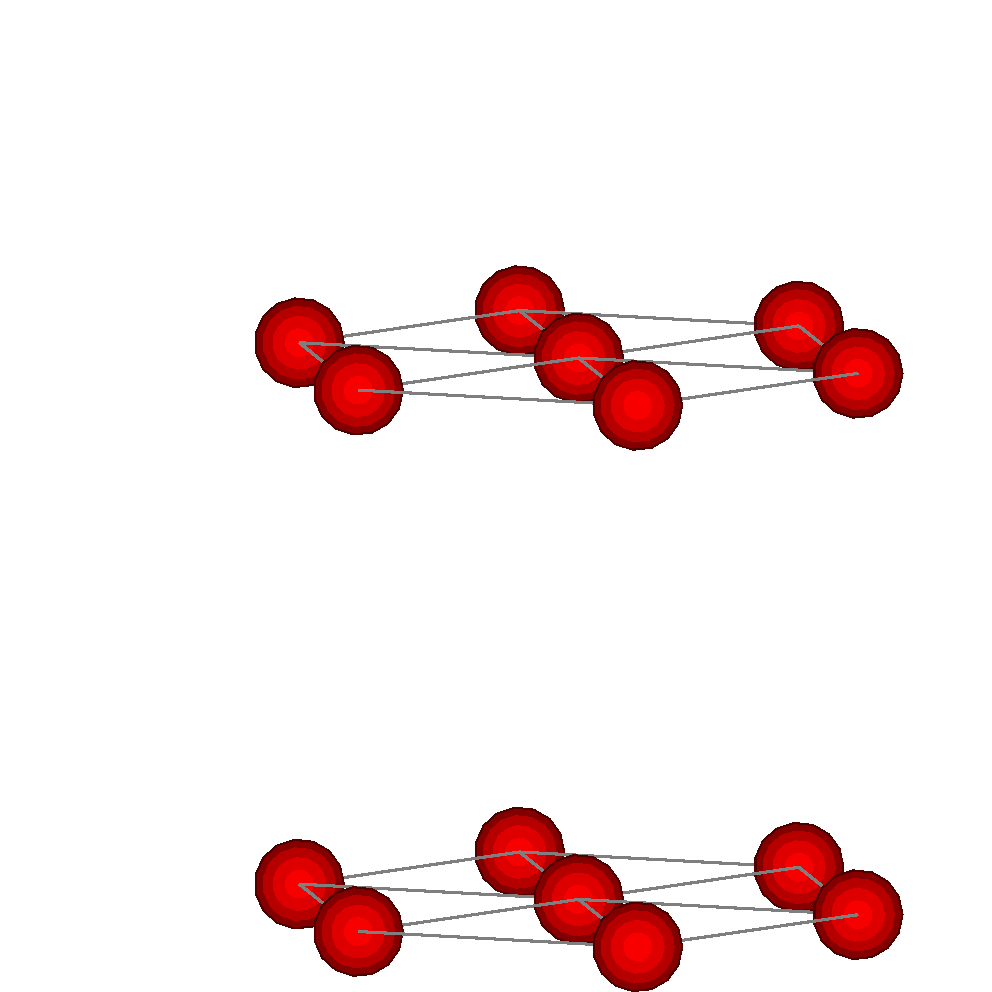
\includegraphics[width=\textwidth]{../assets/hex}
		\caption{hexagonal lattice}
		\label{hex}
	\end{subfigure}
	\begin{subfigure}
		[t]{0.3\textwidth}
		\centering
		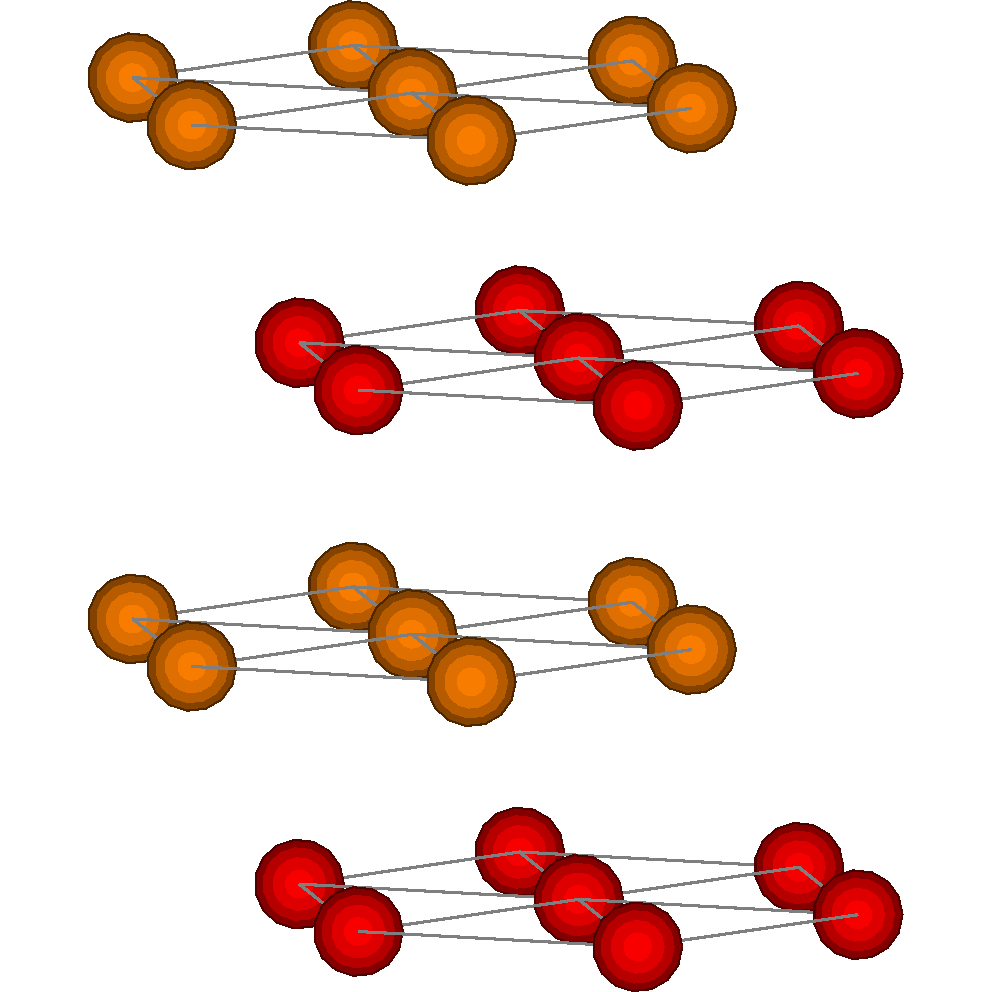
\includegraphics[width=\textwidth]{../assets/hcp}
		\caption{hcp lattice}
		\label{hcp}
	\end{subfigure}
	\par
	\begin{subfigure}
		[t]{0.3\textwidth}
		\centering
		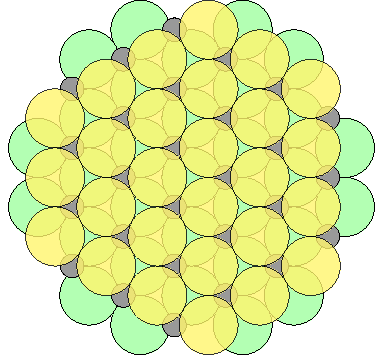
\includegraphics[width=\textwidth]{../assets/corundum_1.pdf}
		\caption{Two oxide layers (green, yellow) with octahedral interstices (gray) between
		them. }
		\label{fig:corundum}
	\end{subfigure}
	\begin{subfigure}
		[t]{0.3\textwidth}
		\centering
		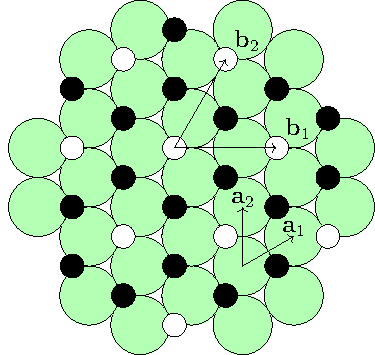
\includegraphics[width=\textwidth]{../assets/corundum_2.pdf}
		\caption{Bottom oxide layer (green) and interstitial mesh with aluminum
		submesh (black).}
		\label{fig:corundum_2}
	\end{subfigure}
	\begin{subfigure}
		[t]{0.3\textwidth}
		\centering
		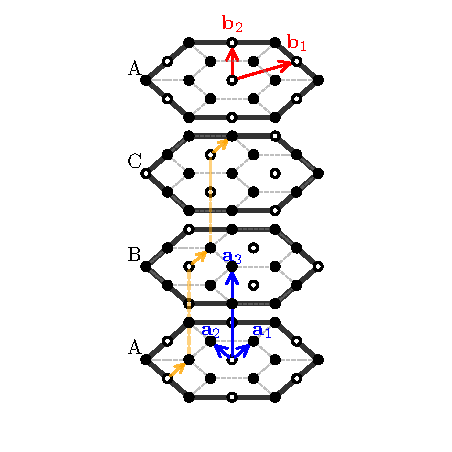
\includegraphics[width=\textwidth]{../assets/corundum_3.pdf}
		\caption{3D view of interstitial meshes with holes (white) and aluminum
		atoms (black).}
		\label{fig:corundum_3}
	\end{subfigure}
	\caption{Selected crystal lattices for investigating the corundum structure\label{fig:lattice_structures}}
\end{figure*}

The sapphire substrate examined in this work crystallizes in the corundum structure,
which was examined by \citeauthoryear{kronberg_plastic_1957}. Understanding it
requires first considering the simple hexagonal structure, defined by the primitive
vectors:
\begin{equation}
	\mathbf{a}_{1}=\frac{a}{2}
	\begin{pmatrix}
		\sqrt{ 3 } \\
		1          \\
		0
	\end{pmatrix}
	\quad \mathbf{a}_{2}=\frac{a}{2}
	\begin{pmatrix}
		\sqrt{ 3 } \\
		-1         \\
		0
	\end{pmatrix}
	\quad \mathbf{a}_{3}=c
	\begin{pmatrix}
		0 \\
		0 \\
		1
	\end{pmatrix}
	\label{eq:hex}
\end{equation}
These vectors create a lattice featuring points at the corners of a hexagon and
at the centers of its hexagonal faces, as shown in \cref{hex}. The hexagonal
close-packed (hcp) structure arises as a simple hexagonal lattice with a two-atom
basis at the lattice positions $(0,0,0)$ and
$(\mathbf{a}_{1}/3 + \mathbf{a}_{2}/3 + \mathbf{a}_{3}/2)$, as shown in \cref{hcp}
\autocite{Ashcroft}.

The sapphire (\ce{Al2O3}) structure features an hcp oxygen sublattice. In this
structure, empty spaces exist between the closely packed oxygen atoms. Since
every empty space is surrounded by six oxygen atoms that form an octahedron, these
spaces are referred to as octahedral interstices and depicted in \cref{fig:corundum}.
The interstices lie on planes midway between two adjacent oxygen hcp layers and
are occupied by aluminum atoms. Since the third hcp layer is directly above the first,
the second interstitial layer is directly above the first. Therefore, all
hexagonal interstitial meshes are above one another, leading to a hexagonal arrangement
of interstices.

\Cref{fig:corundum_2} displays the arrangement of aluminum atoms in the in-plane interstitial
hexagonal mesh. Since the number of interstices corresponds to the number of the
oxygen layer below and since the stoichiometry of aluminum oxide is $\ce{Al2O3}$,
2/3 of these interstices are occupied by aluminum atoms. The remaining 1/3 of
the interstices are empty and are called holes. These holes are regions of negative
localized charge. The requirement of an ordered aluminum sublattice leads to an
in-plane solution maximizing the hole separation due to their negative charge. To
fulfill this condition in-plane, the holes are arranged in a wider hexagonal "hole"
mesh as a subset of the interstitial mesh, shown in \cref{fig:corundum_2}.

The arrangement of holes between adjacent meshes is not arbitrary. Requiring an
ordered sublattice with maximum separation between the holes uniquely determines
the arrangement. The holes in adjacent meshes are shifted relative to each other along
the close-packed direction of the oxygen hcp lattice by a magnitude of an oxygen-oxygen
distance. This out-of-plane shift of the holes is depicted in
\cref{fig:corundum_3}. Since a translation of three out-of-plane shift vectors results
in an identical arrangement, three different hole layers exist, labeled A, B, and
C. The oxygen hcp meshes are labeled with '1' and '2'. The structural repeat unit
of the corundum structure is then given by the sequence 1A2B1C2A1B2C consisting of
six oxygen layers.

The corundum structure is illustrated using \ce{Al2O3} as a representative
material, with reference to the hcp oxygen sublattice and an alumuminum intersticial
mesh, though this may in general be substituted by other anions/cations. \ac{algao}
also crystallizes in corundum structure, where Al and Ga occupy the interstitial lattice
\autocite{peelaers_structural_2018}.

\subsection{Reciprocal Space}
\label{sec:reciprocal_space}

The reciprocal lattice is an important concept in the subsequent considerations of
periodic structures. The goal is to construct a function that is lattice-periodic
in the direct lattice. This function should therefore satisfy $f(\mathbf{x})=f(\mathbf{x}
+\mathbf{A})$, if $\mathbf{A}=\sum_{i=1}^{3}\alpha_{i}\mathbf{a}_{i}$. Using a series
expansion, the following form is obtained:
\begin{align}
	f(\mathbf{x})            & =\sum_{\mathbf{B}}a_{\mathbf{B}}\cdot \exp(\mathrm{i}\mathbf{B}\cdot\mathbf{x}), \notag                                                                                                                  \\
	f(\mathbf{x}+\mathbf{A}) & =\sum_{\mathbf{B}}a_{\mathbf{B}}\cdot \exp(\mathrm{i}\mathbf{B}\cdot \mathbf{x})\cdot \notag \underbrace{ \exp(\mathrm{i}\mathbf{B}\cdot \mathbf{A}) }_{ \stackrel{!}{=}1 }\stackrel{!}{=}f(\mathbf{x}).
\end{align}
This implies the necessary condition $\exp(\mathrm{i}\mathbf{B}\cdot \mathbf{A})=
1$, that is equivalent to $\mathbf{B}\cdot \mathbf{A}=2\pi z$ with
$z \in \mathbb{Z}$. It is possible to define the reciprocal lattice by the set $\{
\mathbf{B}\,\vert\, \exp(\mathrm{i}\mathbf{B}\cdot \mathbf{A})=1 \quad \forall \mathbf{A}
\in \text{span}(\mathbf{a}_{i}) \}$ \autocite{Ashcroft}. Analogous to real space,
primitive vectors can also be formed as:
\begin{equation}
	\mathbf{b}_{1}= 2\pi \cdot \frac{\mathbf{a}_{2}\times \mathbf{a}_{3}}{V_{\mathrm{UC}}}
	\quad \mathbf{b}_{2}= 2\pi \cdot \frac{\mathbf{a}_{3}\times \mathbf{a}_{1}}{V_{\mathrm{UC}}}
	\quad \mathbf{b}_{3}= 2\pi \cdot \frac{\mathbf{a}_{1}\times \mathbf{a}_{2}}{V_{\mathrm{UC}}}
	. \label{eq:reciprocal_vectors}
\end{equation}
Every point in the reciprocal lattice can be described by $\sum_{i=1}^{3}\beta_{i}
\mathbf{b}_{i}$ with $\beta_{i}\in \mathbb{Z}, i\in\{1,2,3\}$. The relation
$\mathbf{b}_{i}\cdot \mathbf{a}_{j}=2 \pi \delta_{ij}$ holds, where $\delta_{ij}$
is the Kronecker delta \autocite{Ashcroft}.

Applying the general construction of \cref{eq:reciprocal_vectors} to the
primitive vectors of the simple hexagonal lattice given in \cref{eq:hex} yields
the reciprocal lattice vectors:
\begin{align}
	\mathbf{b}_{1}=\frac{2\pi}{\sqrt{ 3 }a}\begin{pmatrix}1 \\ \sqrt{ 3 } \\ 0\end{pmatrix} \quad \mathbf{b}_{2}=\frac{2\pi}{\sqrt{ 3 }a}\begin{pmatrix}1 \\ -\sqrt{ 3 } \\ 0\end{pmatrix} \quad \mathbf{b}_{3}= \frac{2\pi}{c}\begin{pmatrix}0 \\ 0 \\ 1\end{pmatrix} \label{eq:hex_reciprocal}
\end{align}
Since $\mathbf{b}_{1}$ and $\mathbf{b}_{2}$ lie in the $xy$-plane while $\mathbf{b}
_{3}$ is parallel to the $c$-axis, the reciprocal lattice of a simple hexagonal
lattice is again hexagonal, but rotated by \ang{30} about the $c$-axis relative
to the direct lattice. The corresponding reciprocal lattice spacings follow directly
from the magnitudes of \cref{eq:hex_reciprocal}:
\begin{equation}
	\lvert \mathbf{b}_{1}\rvert =\lvert \mathbf{b}_{2}\rvert = \frac{4\pi}{\sqrt{3}a}
	\quad \lvert \mathbf{b}_{3}\rvert =\frac{2\pi}{c}
\end{equation}

\subsection{Lattice Planes and Directions}
\label{sec:lattice_planes_and_directions}
This section is based on the findings of \citeauthoryear{Ashcroft}.

An important application of the reciprocal lattice is the characterization of
lattice planes. A lattice plane is any plane lying in the direct lattice that contains
at least three non-collinear lattice points. Due to crystal symmetry, infinitely many
other lattice points lie within this plane. Using translational symmetry, one can
find parallel lattice planes separated by a distance $d$. These are grouped
together as families of lattice planes.

Families of lattice planes can be characterized using the reciprocal lattice, because
for every family with spacing $d$, there exist vectors of the reciprocal lattice
that are perpendicular to the planes. For a unique description, the shortest of
these vectors, $\mathbf{b}$, is chosen, which always has the length $2 \pi / d$.
The converse is also true: for every vector $\mathbf{B}$ from the reciprocal lattice,
there exists a family of perpendicular lattice planes. The spacing $d$ of these planes
is linked to the magnitude of the smallest vector $\mathbf{b}$ parallel to $\mathbf{B}$
by $\lvert \mathbf{b}\rvert=2\pi /d$. Thus, there is a simple way to uniquely identify
lattice planes using reciprocal lattice vectors.

To label families of lattice planes, Miller indices are used. Let $\mathbf{b}$ be
the shortest reciprocal lattice vector perpendicular to the plane being characterized.
This can be represented as
$\mathbf{b}= h \mathbf{b_1}+ k \mathbf{b_2}+ l \mathbf{b_3}$. The tuple $(h\,k\,l
)$ are the Miller indices, which by definition must be integers.

There is a geometric interpretation that allows the indices to be visualized in
real space. For every lattice plane, a corresponding $A \in \mathbb{R}$ can be
found such that the plane equation $\mathbf{b}\cdot \mathbf{x}= A$ is satisfied. By
defining the intercepts of the plane with the coordinate axes spanned by the primitive
vectors $\mathbf{a}_{i}$ as $x_{1}\mathbf{a}_{1}, x_{2}\mathbf{a}_{2}, x_{3}\mathbf{a}
_{3}$, the plane equation $\mathbf{b}\cdot (x_{i}\mathbf{a}_{i})=A$ is satisfied,
and with $\mathbf{b}\cdot \mathbf{a}_{1}=2\pi h$,
$\mathbf{b}\cdot \mathbf{a}_{2}=2\pi k$, $\mathbf{b}\cdot \mathbf{a}_{3}=2\pi l$,
the following relationship is obtained:
\begin{equation}
	x_{1}=\frac{A}{2\pi h}, \quad x_{2}=\frac{A}{2\pi k}, \quad x_{3}=\frac{A}{2\pi
	l}.
\end{equation}
If the axial intercepts $x_{i}$ are known, the Miller indices can be found by
choosing the smallest possible parameter $A$ such that $h$, $k$, and $l$ are
integers.

Lattice directions can be indexed in a similar way. The tuple $[u \,v \,w]$ describes
the direction given by the vector $\mathbf{a}= u\mathbf{a}_{1}+v\mathbf{a}_{2}+ w
\mathbf{a}_{3}$. It should be noted that direction vectors in this context exist
in real space, whereas plane normal vectors are represented by vectors in reciprocal
space. To emphasize this, square brackets are used instead of parentheses.
Furthermore, a special notation exists to denote equivalent families of lattice planes
and directions. In this context, this means that it is possible to transform equivalent
families of planes and directions into one another through symmetry operations.
Equivalent planes are denoted by $\{h\,k\,l\}$, and for directions,
$\langle u\,v\,w\rangle$ is used accordingly.

\subsection{Real Crystals}
\begin{figure*}
	\centering
	\begin{subfigure}
		{0.3\linewidth}
		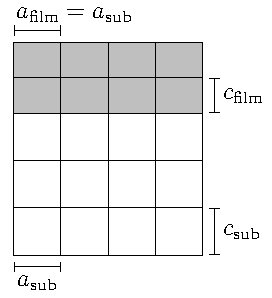
\includegraphics{../assets/pseudomorphic.pdf}
		\caption{Pseudomorphic growth of a thin film on a substrate}
	\end{subfigure}
	\begin{subfigure}
		{0.3\linewidth}
		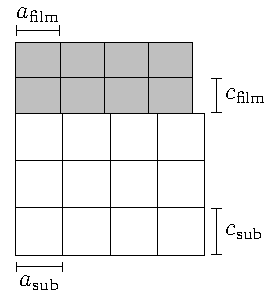
\includegraphics{../assets/partially_relaxed.pdf}
		\caption{Partially relaxed thin film on a substrate}
	\end{subfigure}
	\begin{subfigure}
		{0.3\linewidth}
		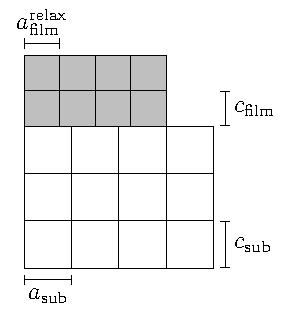
\includegraphics{../assets/fully_relaxed.pdf}
		\caption{Fully relaxed thin film on a substrate}
	\end{subfigure}
	\caption{Heteroepitaxial thin film growth. }
	\label{fig:film_growth}
\end{figure*}

As the crystal is in energy exchange with its environment, it minimizes the free
energy $F=U-TS$ instead of its internal energy $U$. This introduces deviations from
the ideal crystal structure, i.e. defects. A small concentration of defects can
fundamentally influence the crystal's properties.

Most thin films differ chemically from their substrate. In that case, the film
grows heteroepitaxially, depicted in \cref{fig:film_growth}. If the lattice
constants do not differ too much, the film adopts the substrate's in-plane lattice
constant $a$. This is called pseudomorphic growth. A figure of merit to quantify the
degree of relaxation is given as:
\begin{equation}
	r = \frac{a_{\mathrm{film}}- a_{\mathrm{substrate}}}{a_{\mathrm{film}}^{\mathrm{relax}}-
	a_{\mathrm{substrate}}}
\end{equation}
In this equation, $a_{\mathrm{film / substrate}}$ is the measured in-plane lattice
constant of a thin film / substrate, and $a_{\mathrm{film}}^{\mathrm{relax}}$ is
the fully relaxed lattice constant. $r=0$ corresponds to pseudomorphic growth,
while $r=1$ corresponds to a fully relaxed film. $r<1$ induces material strain.

As the strain of the film increases with each deposited layer, strain energy is
released by one-dimensional defects: dislocations. The dislocation's orientation
is characterized by a dislocation vector $\mathbf{L}$. Most of the time,
dislocations appear parallel to the growth direction. By moving in a loop around the
dislocation using the local lattice coordinate system, the starting point is not
reached. The difference between start and end point is defined by the Burgers vector
$\mathcal{B}$, depicted in \cref{fig:dislocations}. Depending on the orientation of
$\mathcal{B}$ relative to $\mathbf{L}$, one can distinguish between screw-type
dislocations ($\mathcal{B}\parallel \mathbf{L}$) and edge-type dislocations ($\mathcal{B}
\perp \mathbf{L}$).

Edge-type dislocations prefer to group together in order to minimize the total
strain energy. This agglomeration of dislocations results in grain boundaries which
separate monocrystalline regions of the thin film, called crystallites. They are twisted
by an angle $\delta$. By analog reasoning, an agglomeration of screw-type dislocations
results in a tilt of the crystallites.

\begin{figure}
	\centering
	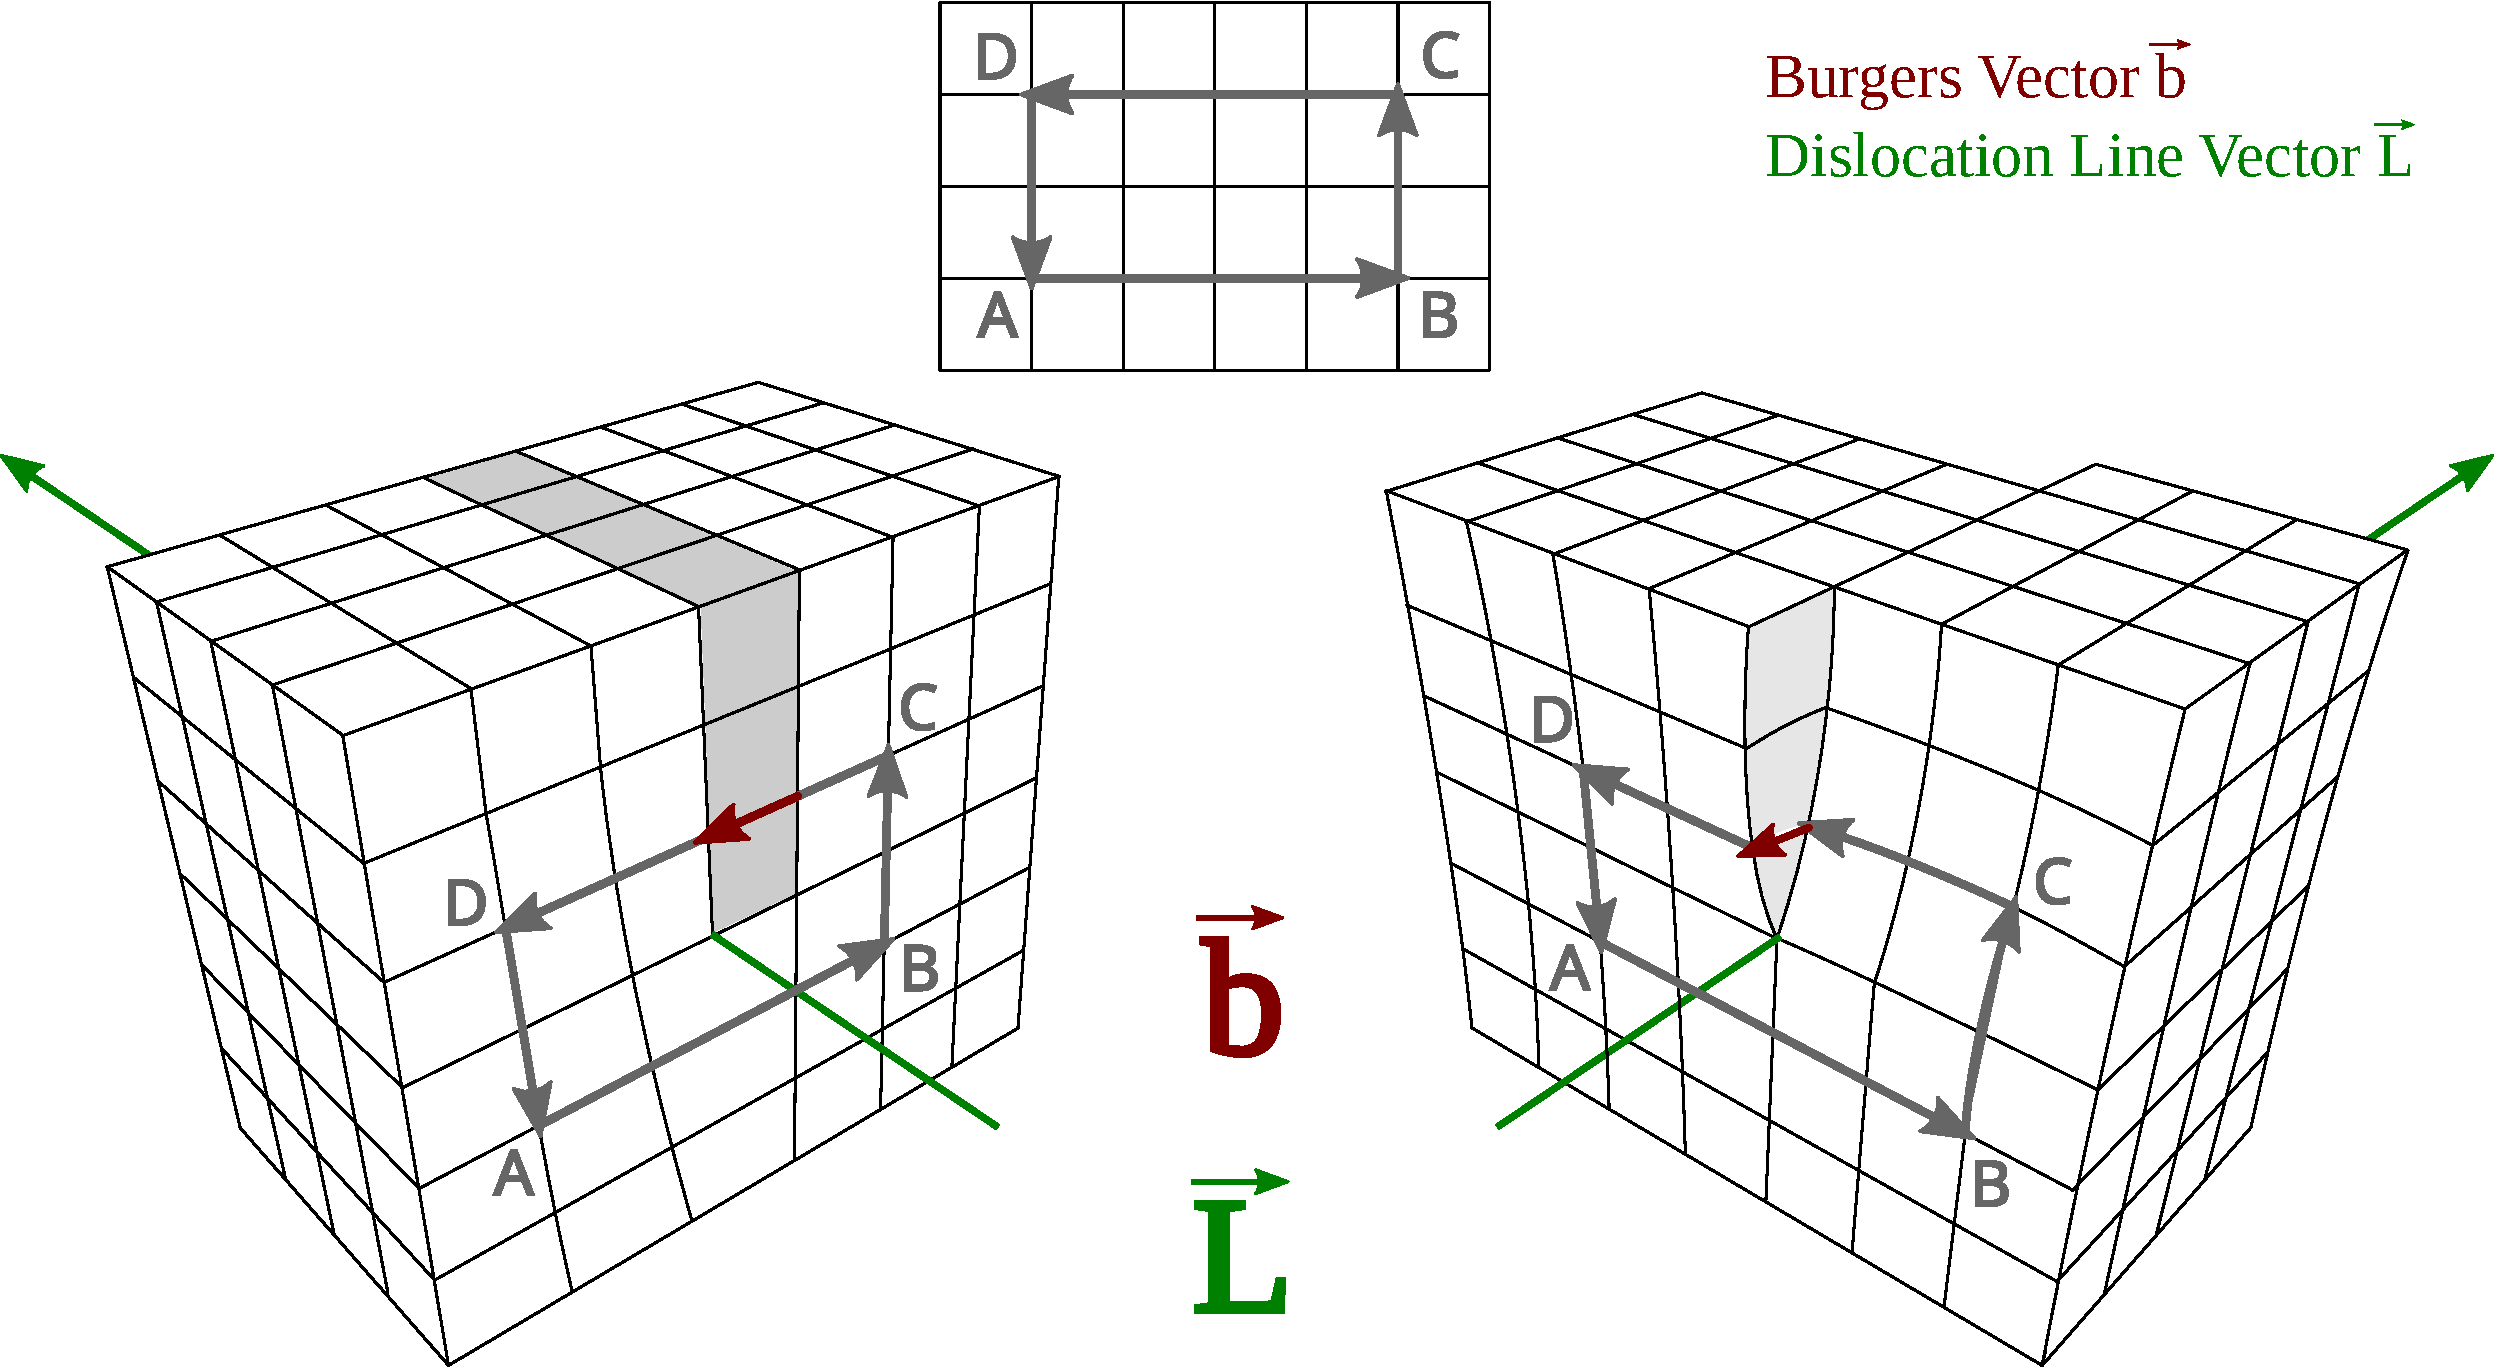
\includegraphics[width=0.7\linewidth]{../assets/dislocation_types.pdf}
	\caption{dislocations of edge (left) and screw (right) type. Burgers vector labeled
	as $\vec{b}$.}
	\label{fig:dislocations}
\end{figure}